%%%%%%%%%%%%%%%%%%%%%%%%%%%%%%%%%%%%%%%%%%%%%%%%%%%%%%%%%%%%%%%%%%%%%%%%
% Plantilla TFG/TFM
% Escuela Politécnica Superior de la Universidad de Alicante
% Realizado por: Jose Manuel Requena Plens
% Contacto: info@jmrplens.com / Telegram:@jmrplens
%%%%%%%%%%%%%%%%%%%%%%%%%%%%%%%%%%%%%%%%%%%%%%%%%%%%%%%%%%%%%%%%%%%%%%%%

\section{Brownian motion}
\label{brownian}

According to Encyclopedia Britannica~\cite{BritannicaBrownian}, \textit{Brownian motion is any of various physical phenomena in which some quantity is constantly undergoing small, random fluctuations.}

It gets its name from Robert Brown, the Scottish botanist  who studied it in the first place, circa 1827, in the context of microscopic particles within the pollen grains suspended in water under the microscope. Brown himself would dismiss the theory that this motion had a biological origin.

Half a century later, in view of the relationship between temperature and Brownian velocity, it was suggested that this phenomenon could be caused by the thermal molecular motion of environment.

If true, this would be the first directly observable proof of the kinetic theory\footnote{According to the kinetic theory, the temperature of a substance is proportional to the average kinetic energy with which the molecules of the substance are moving or vibrating: $T=\frac{2}{3} \frac{K}{N k_{B}}$, where $N$ is the number of molecules, $K=\frac{1}{2} N m \overline{v}^{2}$ is the kinetic energy of the system, and $k_{B} = 1.380649 \times 10^{-23} \; \textrm{J/K}$ is the Boltzmann constant}, developed in the late 19th century by Maxwell, Boltzmann and Clausius.

In the beginning of the 20th century, Einstein and Smoluchowski separately produced their quantitative theories of Brownian motion. 

A few years later, the verification of Einstein's model by Jean Perrin would finally demonstrate the atomic nature of matter.

\subsection{From Brownian motion to diffusion}

If in a given medium, the random motion of its particles has no preferred direction, then as time passes, the particles will tend to be spread evenly throughout it.

This process can also be interpreted as a subtance spreding from regions of high concentration to regions of lower concentration, and it is called diffusion. Hence, diffusion can be considered an emergent manifestation on a macrospic level of particles subject to Brownian motion on the microscopic level.

Einsten developed a model based on probability theory that shows that the density of Brownian particles $\rho$ at a point $x$ at time t satisfies the diffusion equation: ???

\begin{equation}
\frac{\partial \rho}{\partial t}=D \frac{\partial^{2} \rho}{\partial x^{2}}
\end{equation}

The solution to this equation, assuming a boundary condition were all particles are at the origin at time t=0 is a normal distribution with mean $\mu=0$ and variance $\sigma^{2}=2 D t$.

Given $\mu=0$, it is possible to conclude that  meaning that a Brownian particle is equally likely to move in any sense and direction.

The second moment\footnote{The $n^{th}$ moment of a real-valued continuous function f(x) of a real variable is defined as:  $\mu_{n}=\int_{-\infty}^{\infty} x^{n} f(x) \mathrm{d} x$} of the distrubution is:

\begin{equation}
\overline{x^{2}}=2 D t
\end{equation}

This allowed Einstein to show that the displacement of a Brownian particle is not proportional to the elapsed time, but rather to its square root.

In a state of dynamic equilibrium, established between concentration driven migration and other present forces, the particle density distribution combined with Fick's Law leads to:

\begin{equation}
D=q k_{\mathrm{B}} T
\end{equation}

where $q = \frac{v}{F_ext}$ is the mobility of a particle in the surrounding fluid, which for a spherical particle with radius $r$ is, as Stokes demonstrated: 

\begin{equation}
q=\frac{1}{6 \pi \mu r}
\end{equation}

Thus, a smaller particle, a less viscous fluid, and a higher temperature would each increase the diffusion coefficient and, therefore, the mean square displacement (MSD). 

\subsection{Influence of microswimmers}

In active suspensions, besides the molecular bombardment, the MSD of Brownian particles can be further enlarged through interactions with the active particles. This interaction can be due to either direct contact or simply to their influence on the flow field.

\begin{figure}[H]
	\centering
	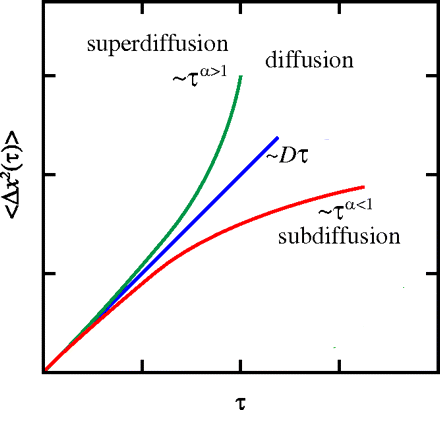
\includegraphics[width=0.4\textwidth]{archivos/SubSuperDif.png}
	\caption{Scaling of the mean square displacement in the scenarios of subdiffusion, diffusion and superdiffusion~\cite{MacKintosh7138} (modified)}
	\label{SSDif}
\end{figure}

Depending on several factors (concentration, elapsed time), the presence of microswimmers can modify the value of the diffusion coefficient (i.e. enlarged gaussian distributions at high concentrations and long times~\cite{Kurtuldu2011}) and even the scaling of the MSD (i.e. modified tails of the distributions at relatively short times~\cite{Kurtuldu2011}). 